\documentclass[12pt]{article}
\usepackage[utf8]{inputenc}
\usepackage{amsmath}
\usepackage{fancyhdr}
\usepackage{graphicx}
\usepackage{epstopdf}

\setlength{\oddsidemargin}{0in}
\setlength{\evensidemargin}{0in}
\setlength{\textwidth}{6.5in}
\setlength{\topmargin}{-.3in}
\setlength{\textheight}{9in}


\pagestyle{fancy}
\begin{document}

\begin{center}
{\Large Machine Learnig Homework 8} \\[.3in]
\end{center}
\lhead{Adam Kosiorek}
\rhead{IMAT: 03661883}
\vspace*{.5in}

\section*{Problem 5}

\begin{figure}[!ht]
 \center
 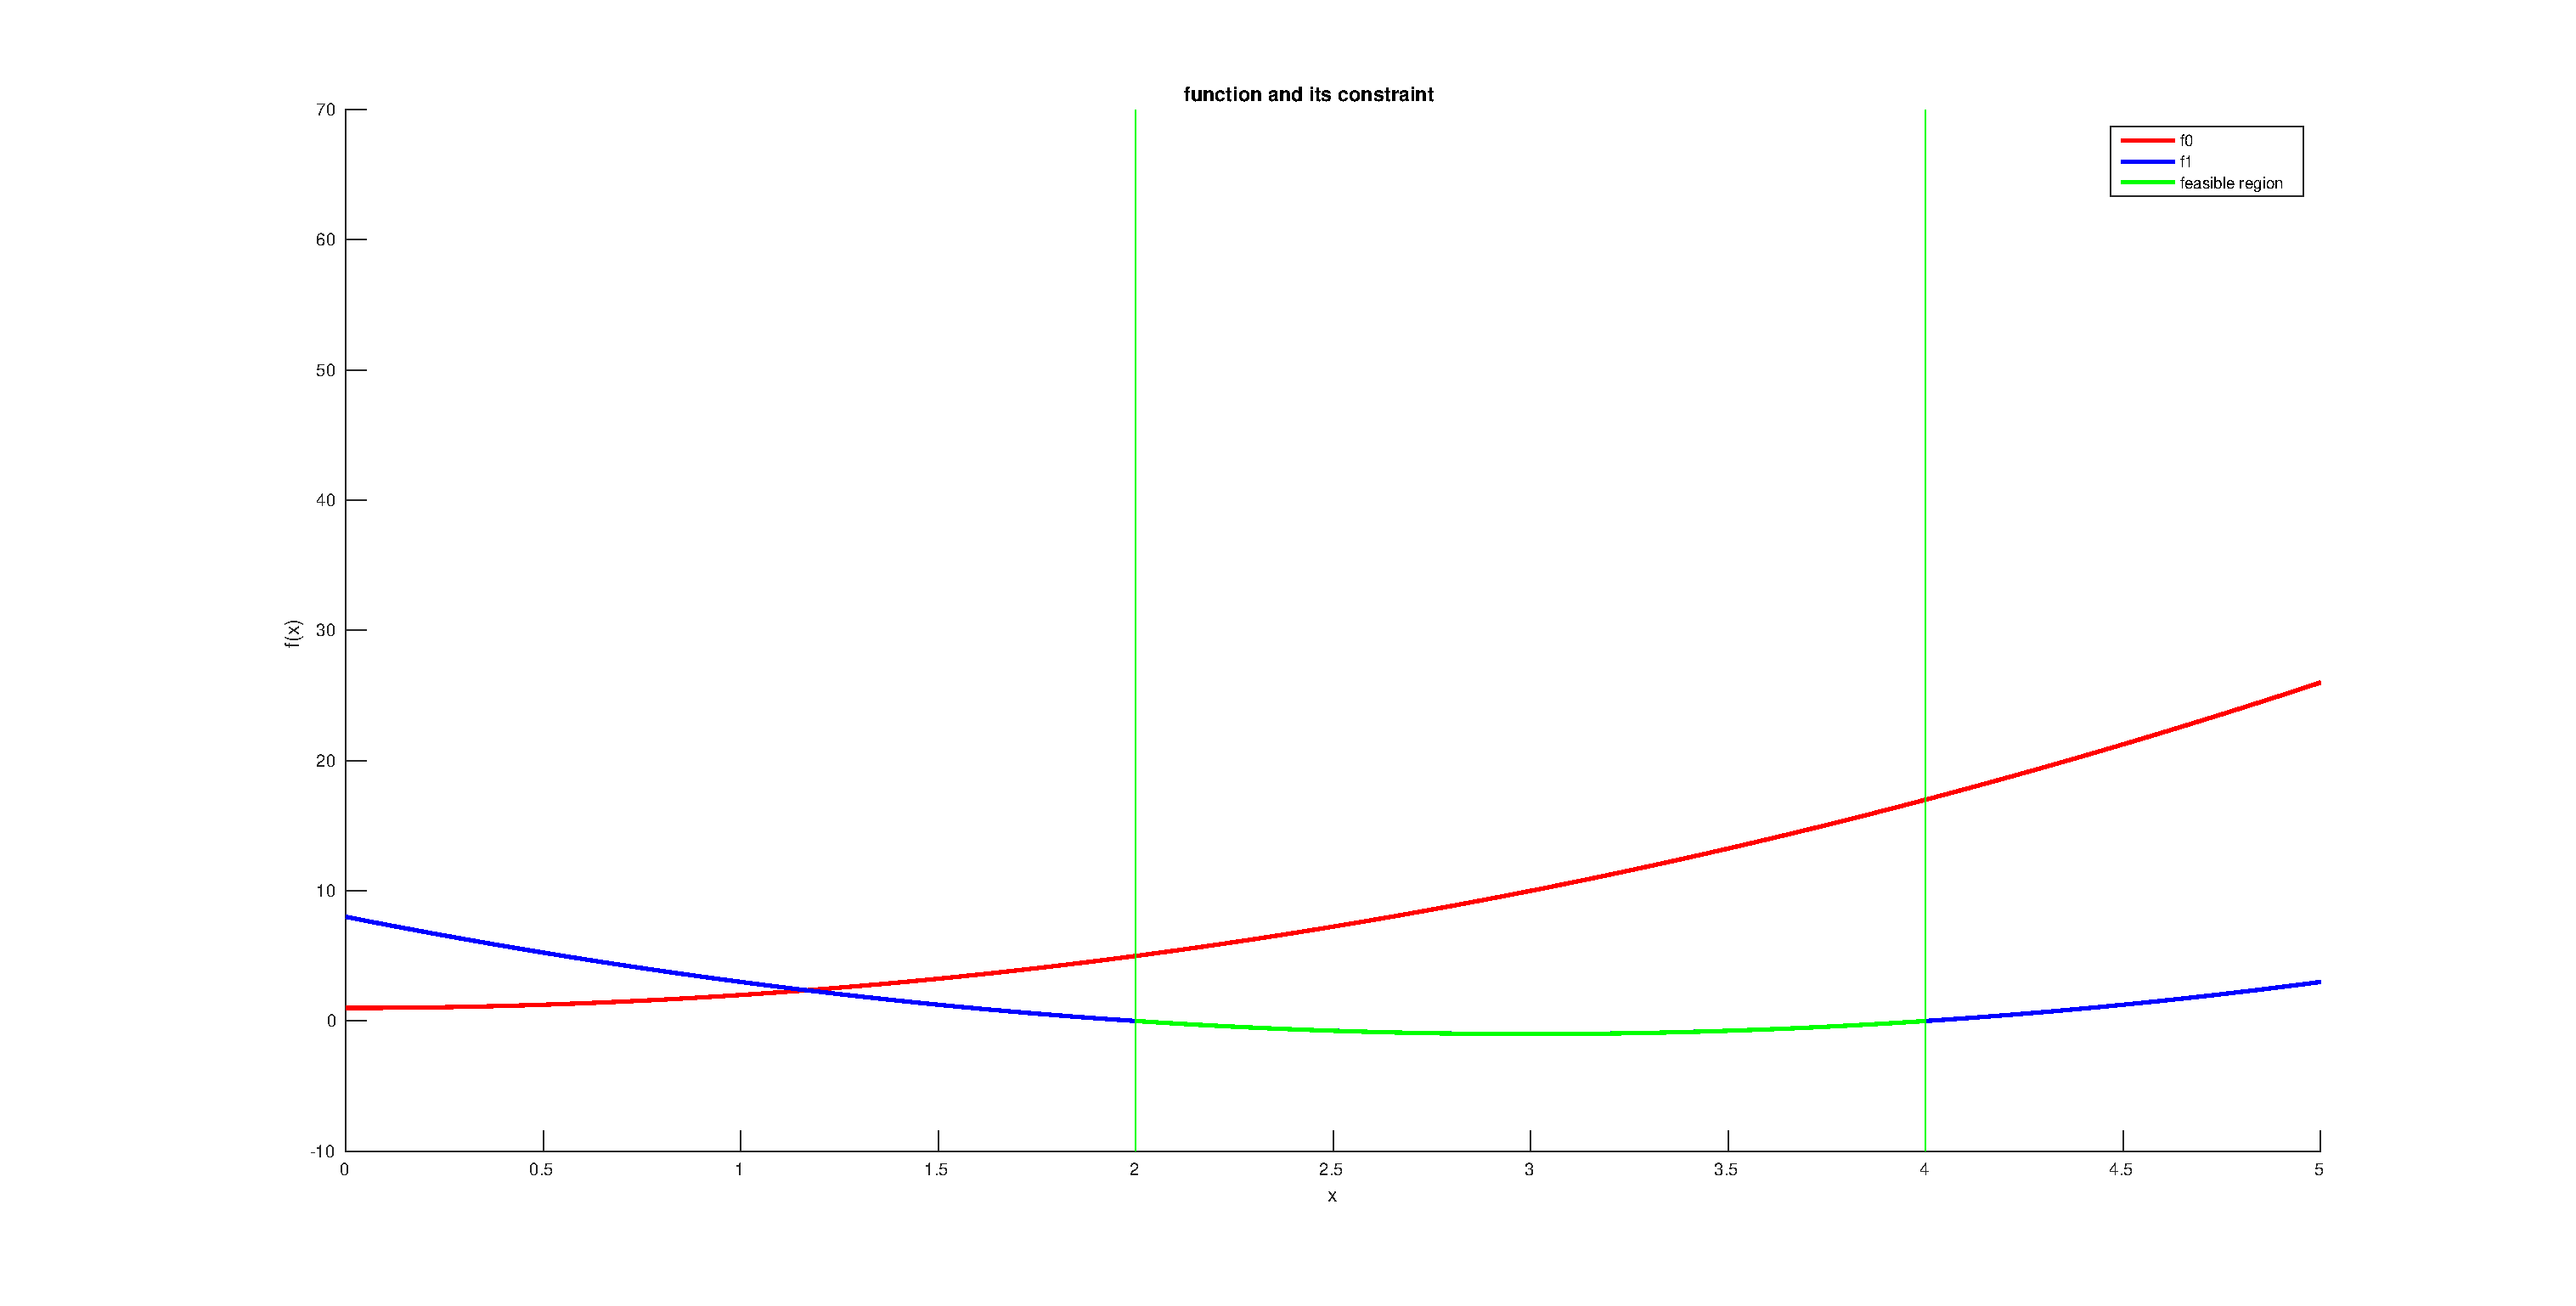
\includegraphics[width=\textwidth]{prob5}
 \label{fig:primal}
\end{figure}

As can be clearly seen in the above plot, $x^\star$ = 2 is the optimal solution.

\section*{Problem 6}

\begin{equation}
 \begin{align}
  L(x, \alpha) &= f_0(x) + \alpha f_1(x) \\
    &= x^2 + 1 + \alpha (x-2)(x-4) \\
    &= (1 + \alpha) x^2 + 6 \alpha x + (1 + 8 \alpha)
 \end{align}
\end{equation}



\begin{figure}[!ht] \label{fig:prob6}
 \center
 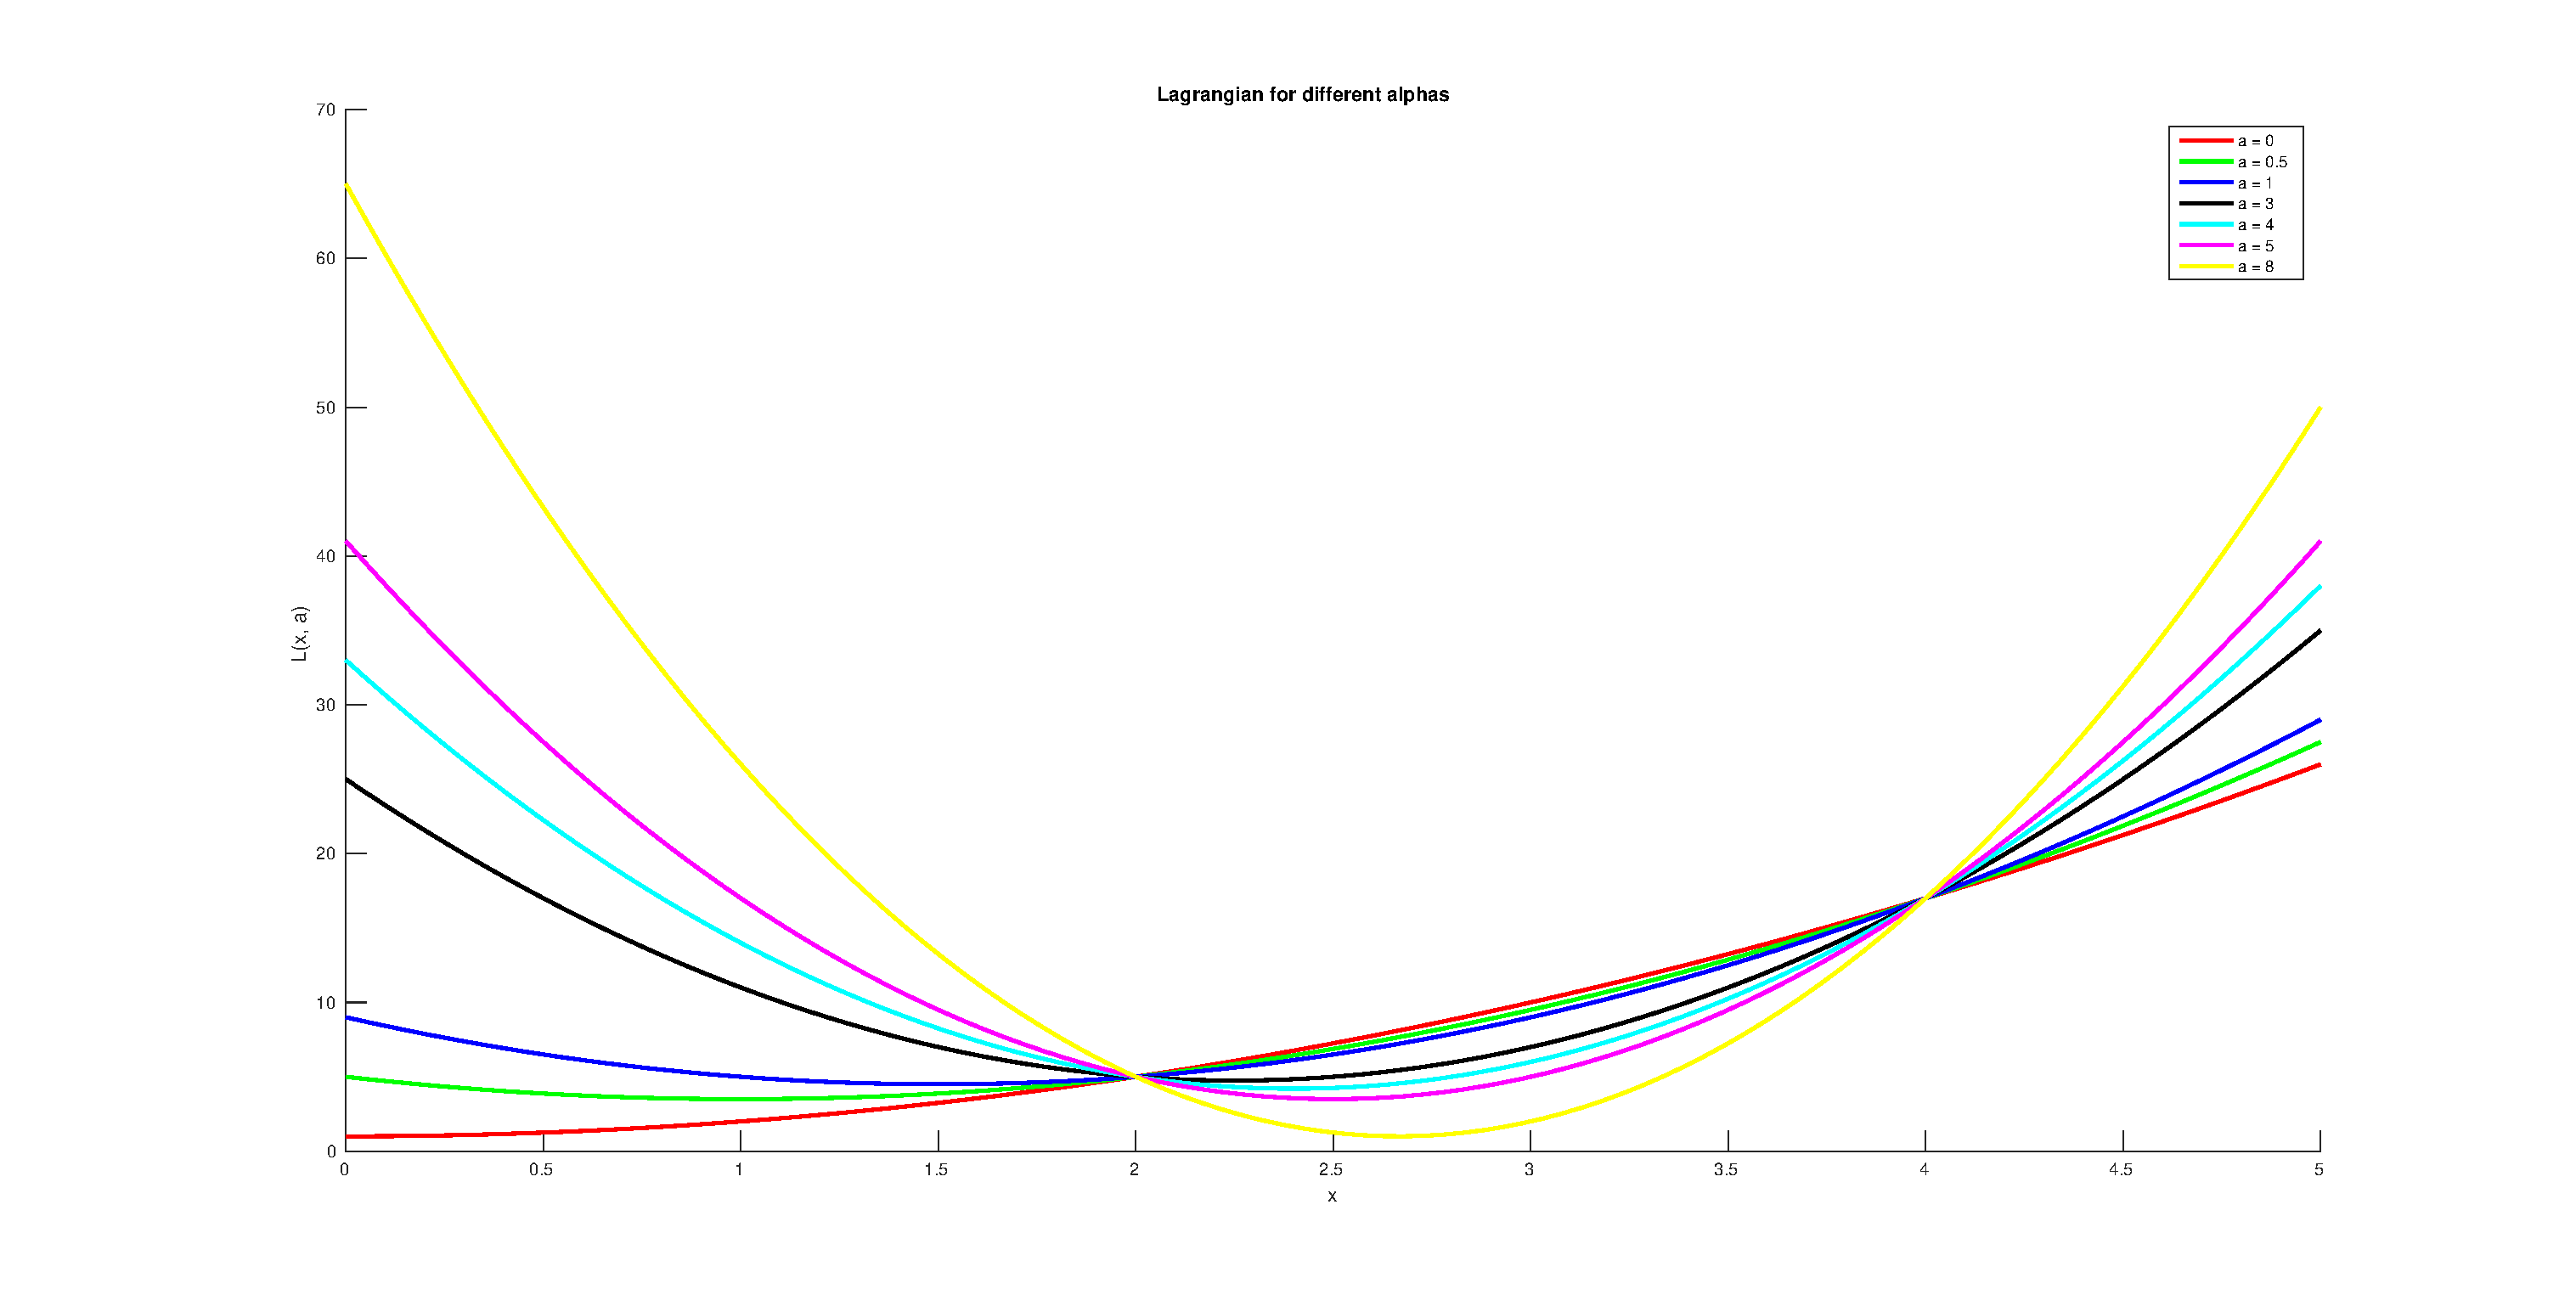
\includegraphics[width=\textwidth]{prob6}
 \caption{Lagrangian $L(x, \alpha)$ for different values of $\alpha$}.
\end{figure}

The value of the objective function is given by the lagrangian $L(x, \alpha)$ evaluated at $\alpha = 0$, portrayed by the red curve in Fig. \ref{fig:prob6}. Lagrangian is smaller than the objective function for $x \in (2, 4)$ and greater than the objective function for $x \notin [2, 4]$. Values at $x = 2$ and $x = 4$ are unaffected by $\alpha$. The upper bound for $\min_x L(x, \alpha) = L(2, \alpha)$ for all $\alpha \geq 0$ is $5$.

\section*{Problem 7}

\begin{equation}
 g(\alpha) = \min_x L(x, \alpha) \implies \frac{\partial}{\partial x} L(x, \alpha) = 0 \implies x^\star = \frac{3 \alpha}{1 + \alpha}
\end{equation}

\begin{equation}
 g(\alpha) = \frac{- \alpha^2 + 9 \alpha + 1}{1 + \alpha}
\end{equation}

The dual problem is plotted in Fig. \ref{fig:dual} and it is given by

\begin{equation}
 \begin{align}
  \max_\alpha g(\alpha) \\
  \text{subject to } \alpha \geq 0
 \end{align}
\end{equation}





\begin{figure}[!ht] \label{fig:dual}
 \center
 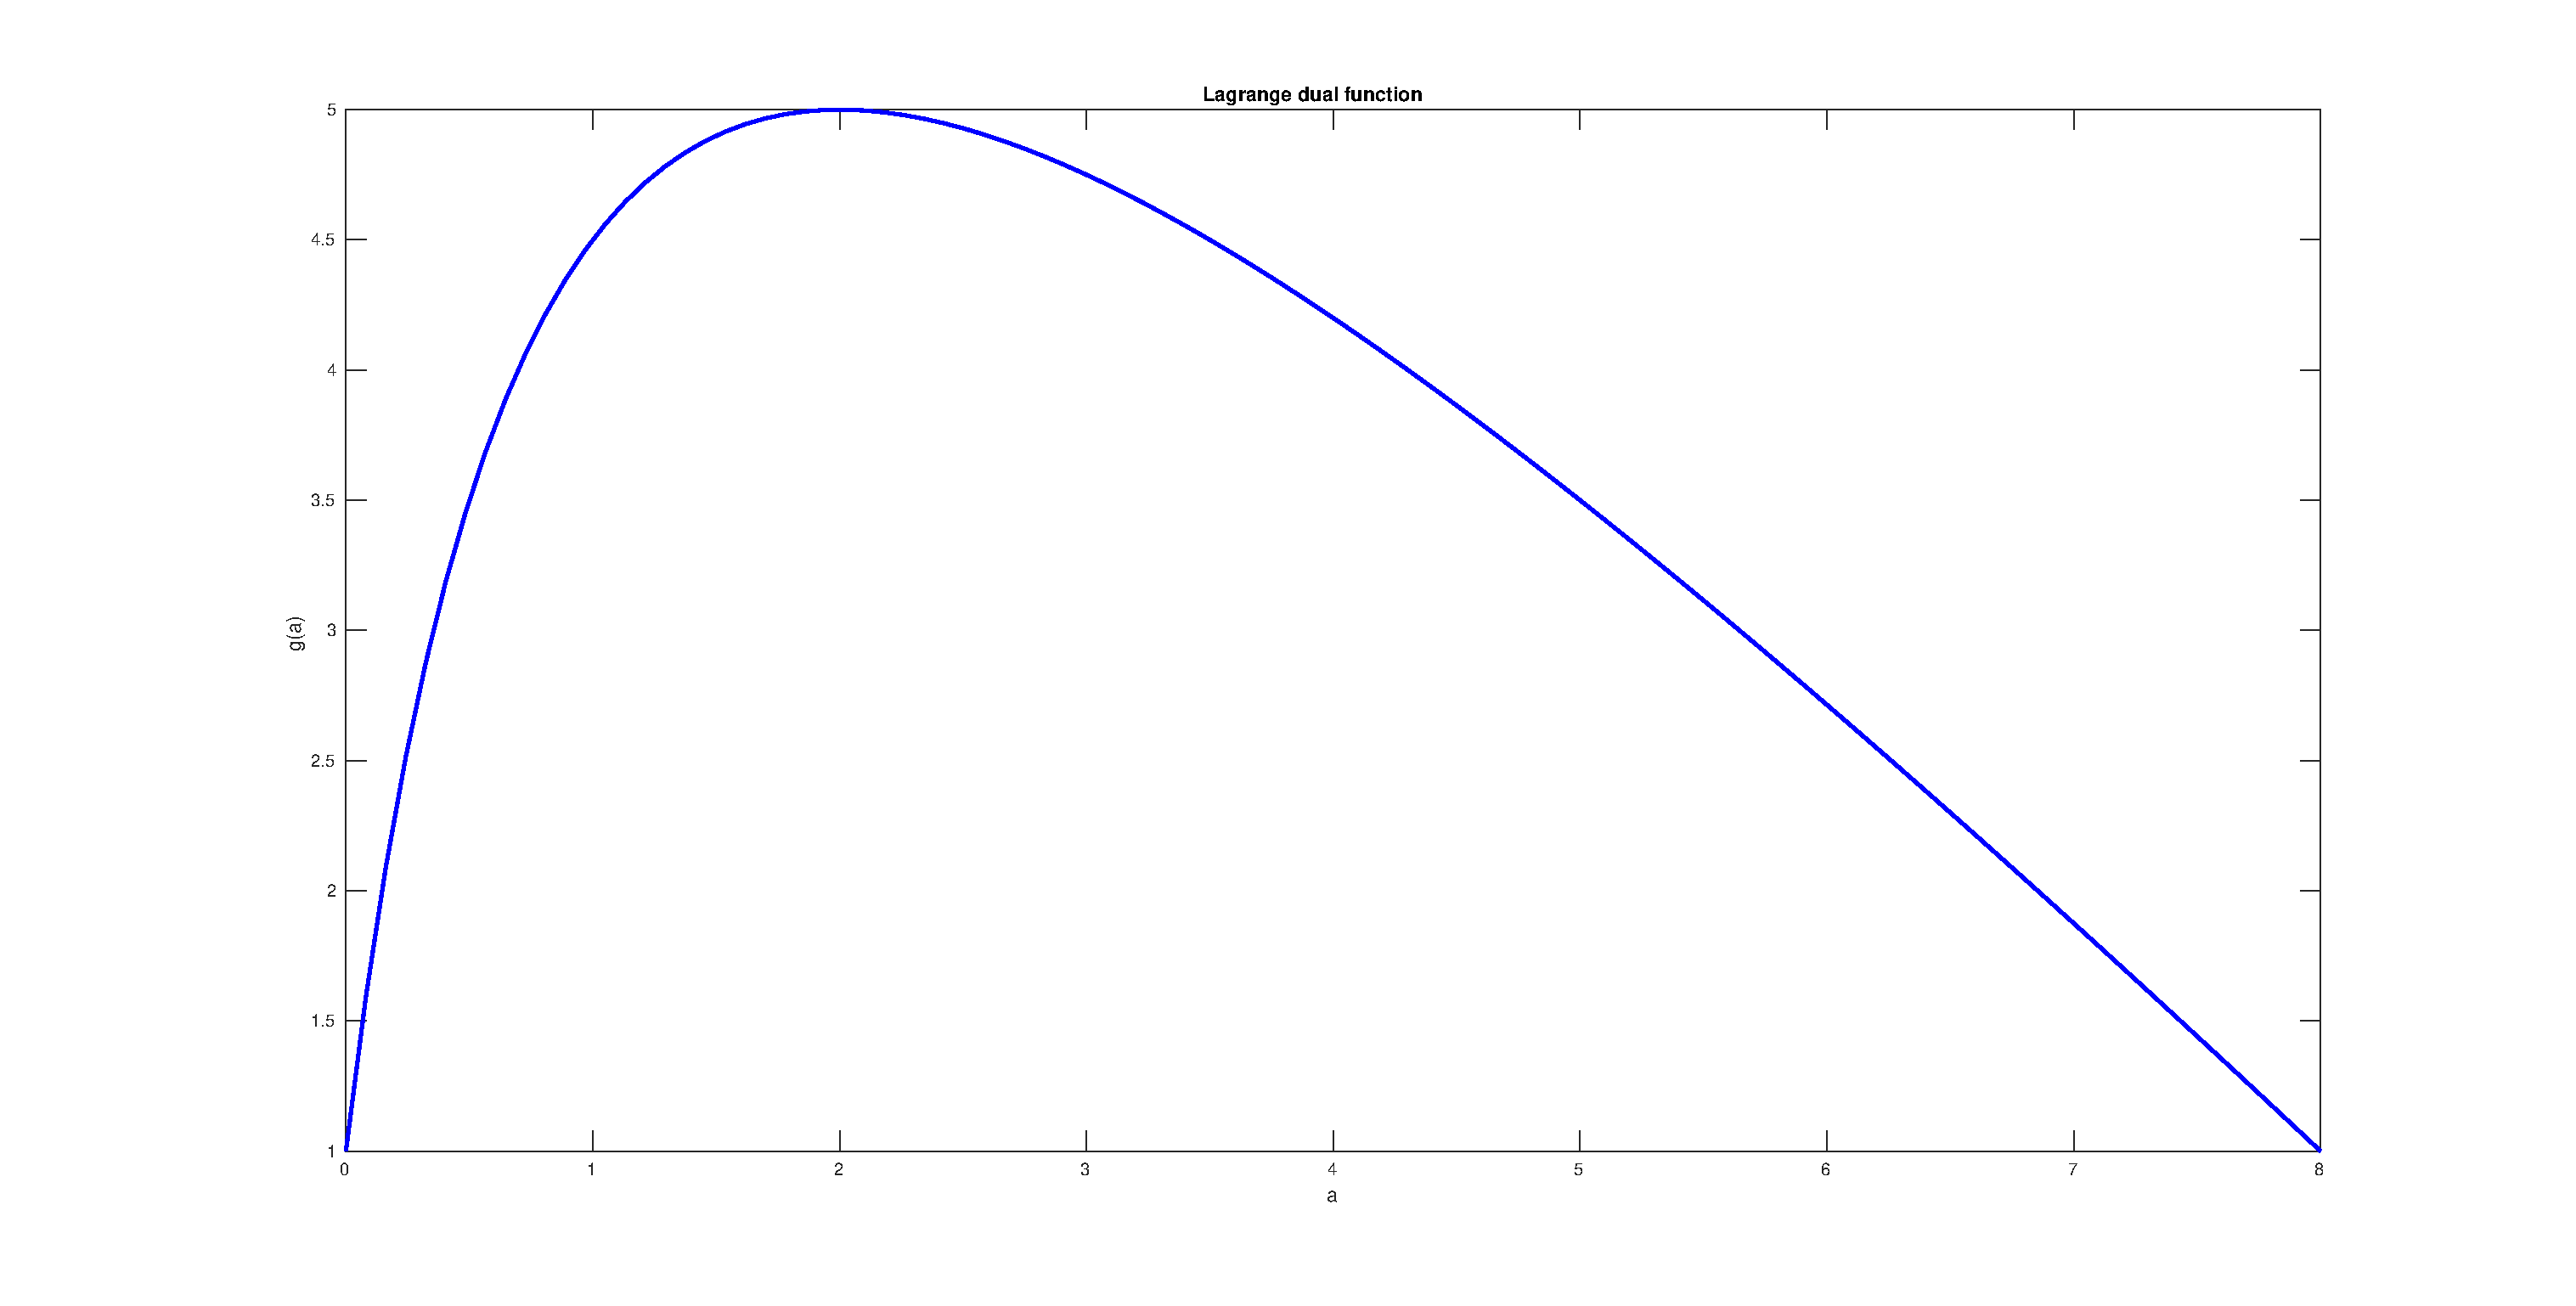
\includegraphics[width=\textwidth]{prob7}
 \caption{Lagrange dual function $g(\alpha)$.}
\end{figure}

\section*{Problem 8}

\begin{equation}
 \alpha^\star = \arg \max_\alpha g(\alpha) 
\end{equation}
\begin{equation}
 0 = \frac{\partial}{\partial \alpha} g(\alpha) = \frac{- \alpha^2 - 2 \alpha +8}{(1 + \alpha)^2} \text{ and } \alpha \geq 0
\end{equation}

The dual optimal solution $\alpha^\star = 2$ and $g(\alpha^\star) = 5$.

\section*{Problem 9}

\begin{equation}
 x^\star = \frac{3 \alpha^\star}{1 + \alpha^\star} = \frac{6}{1 + 2} = 2
\end{equation}

The optimal solution is given by $f_0(x^\star) = 5$, which is equal to the dual optimal value.

\section*{Problem 10}

The constraint $f_1$ is active. We can see it also on the plot of the primal problem in Fig. \ref{fig:primal}, since the feasible region is bounded by the zero-crossings of this constraint and the objective function attains its minimum at one of them.

  
\end{document}
